\section{Result Analysis}
\label{sec:ResultAnalysis}

%comparar as duas cenas
%introduzir o octave optimizado, seguindo a linha de raciocinio do ngspice
%comparar as tabelinhas de output dos dois lados, expicar porque diferem.

\indent

In this section the results will firstly be analysed and then compared, identifying the differences between the {\it Octave} computed results and the {\it Ngspice} simulation results. 

To compare both models, graphs and tables extracted from both sources are going to be analysed and discussed.

In this assignment, the match between the theoretical ({\it Octave}) and the simulated ({\it Ngspice}) models was not as good as usual. This fact could be attributed to the lack of refinement in the {\it Octave} model, which introduced some discrepancies and lowered the precision of the predicted values. 

For all effects, the {\it Ngspice} results should be considered as the most accurate and reliable, for this assignment. 

\subsection{Operating point analysis}

In the following tables the results from the operating point analysis obtained with \textit{Octave} (table \ref{tab:OPOc}) and \textit{Ngspice} (table \ref{tab:OPNG}) are shown.

\begin{table}[H]
    \caption{OP analysis}
    \begin{subtable}{.5\linewidth}
      \centering
        \caption{Octave}
        \begin{tabular}{ll}
        \hline    
        {\bf Name} & {\bf Value} \\ \hline
        \input{../Analysis/OPResults.tex}
        \end{tabular}
        \label{tab:OPOc}
    \end{subtable}%
    \begin{subtable}{.5\linewidth}
      \centering
        \caption{Ngspice}
        \begin{tabular}{ll}
        \hline    
        {\bf Name} & {\bf Value} \\ \hline
        @gcs[i] & 1.837491e-04\\ \hline
@id[current] & 1.033653e-03\\ \hline
@r1[i] & 1.924024e-04\\ \hline
@r2[i] & 1.837491e-04\\ \hline
@r3[i] & 8.653299e-06\\ \hline
@r4[i] & -1.14368e-03\\ \hline
@r5[i] & 8.499042e-04\\ \hline
@r6[i] & 9.512771e-04\\ \hline
@r7[i] & 9.512771e-04\\ \hline
v(1) & 5.008942e+00\\ \hline
v(2) & 4.811140e+00\\ \hline
v(3) & 4.437766e+00\\ \hline
v(4) & 0.000000e+00\\ \hline
v(5) & 4.785125e+00\\ \hline
v(6) & 2.133477e+00\\ \hline
v(7) & -1.98683e+00\\ \hline
v(8) & -2.93853e+00\\ \hline

        \end{tabular}
        \label{tab:OPNG}
    \end{subtable} 
    \label{tab:OP}
\end{table}
\indent

As seen, the values, although close, do not correspond. The values that differ the most are the base voltage ones. This difference comes from errors due to the multiple approximations used in the theoretical analysis such as the transistor model (the behaviour of a transistor was approximated several times). 

\subsection{Frequency analysis}

On the graphics shown below its possible to analyse the bandwidth of the signals that can be amplified: 

\subsubsection*{Graphs}

\begin{figure}[H]
\centering
\begin{subfigure}{.48\textwidth}
  \centering
  \includegraphics[width=.9\linewidth]{Mag_oc.eps}
  \caption{Octave}
  \label{fig:MagOC}
\end{subfigure}%
\begin{subfigure}{.48\textwidth}
  \centering
  \includegraphics[width=.7\linewidth, trim={2cm 1.5cm 0.5cm 6cm}, clip]{../Simulation/vo2f_m.pdf}
  \caption{Ngspice}
  \label{fig:MagNG}
\end{subfigure}
\caption{Magnitude output}
\label{fig:Mag}
\end{figure}

By analysing the graphics it may be concluded that the maximum gains match, although the bandwidths are different. This difference may come from various factors which will be specified further down in the section. A better result can be seen in the simulation values as the input values were optimised looking at the simulation results. \bigskip

Next up are the phase graphics:

\begin{figure}[H]
\centering
\begin{subfigure}{.48\textwidth}
  \centering
  \includegraphics[width=.9\linewidth]{Phase_oc.eps}
  \caption{Octave}
  \label{fig:PhaOC}
\end{subfigure}
\begin{subfigure}{.48\textwidth}
  \centering
  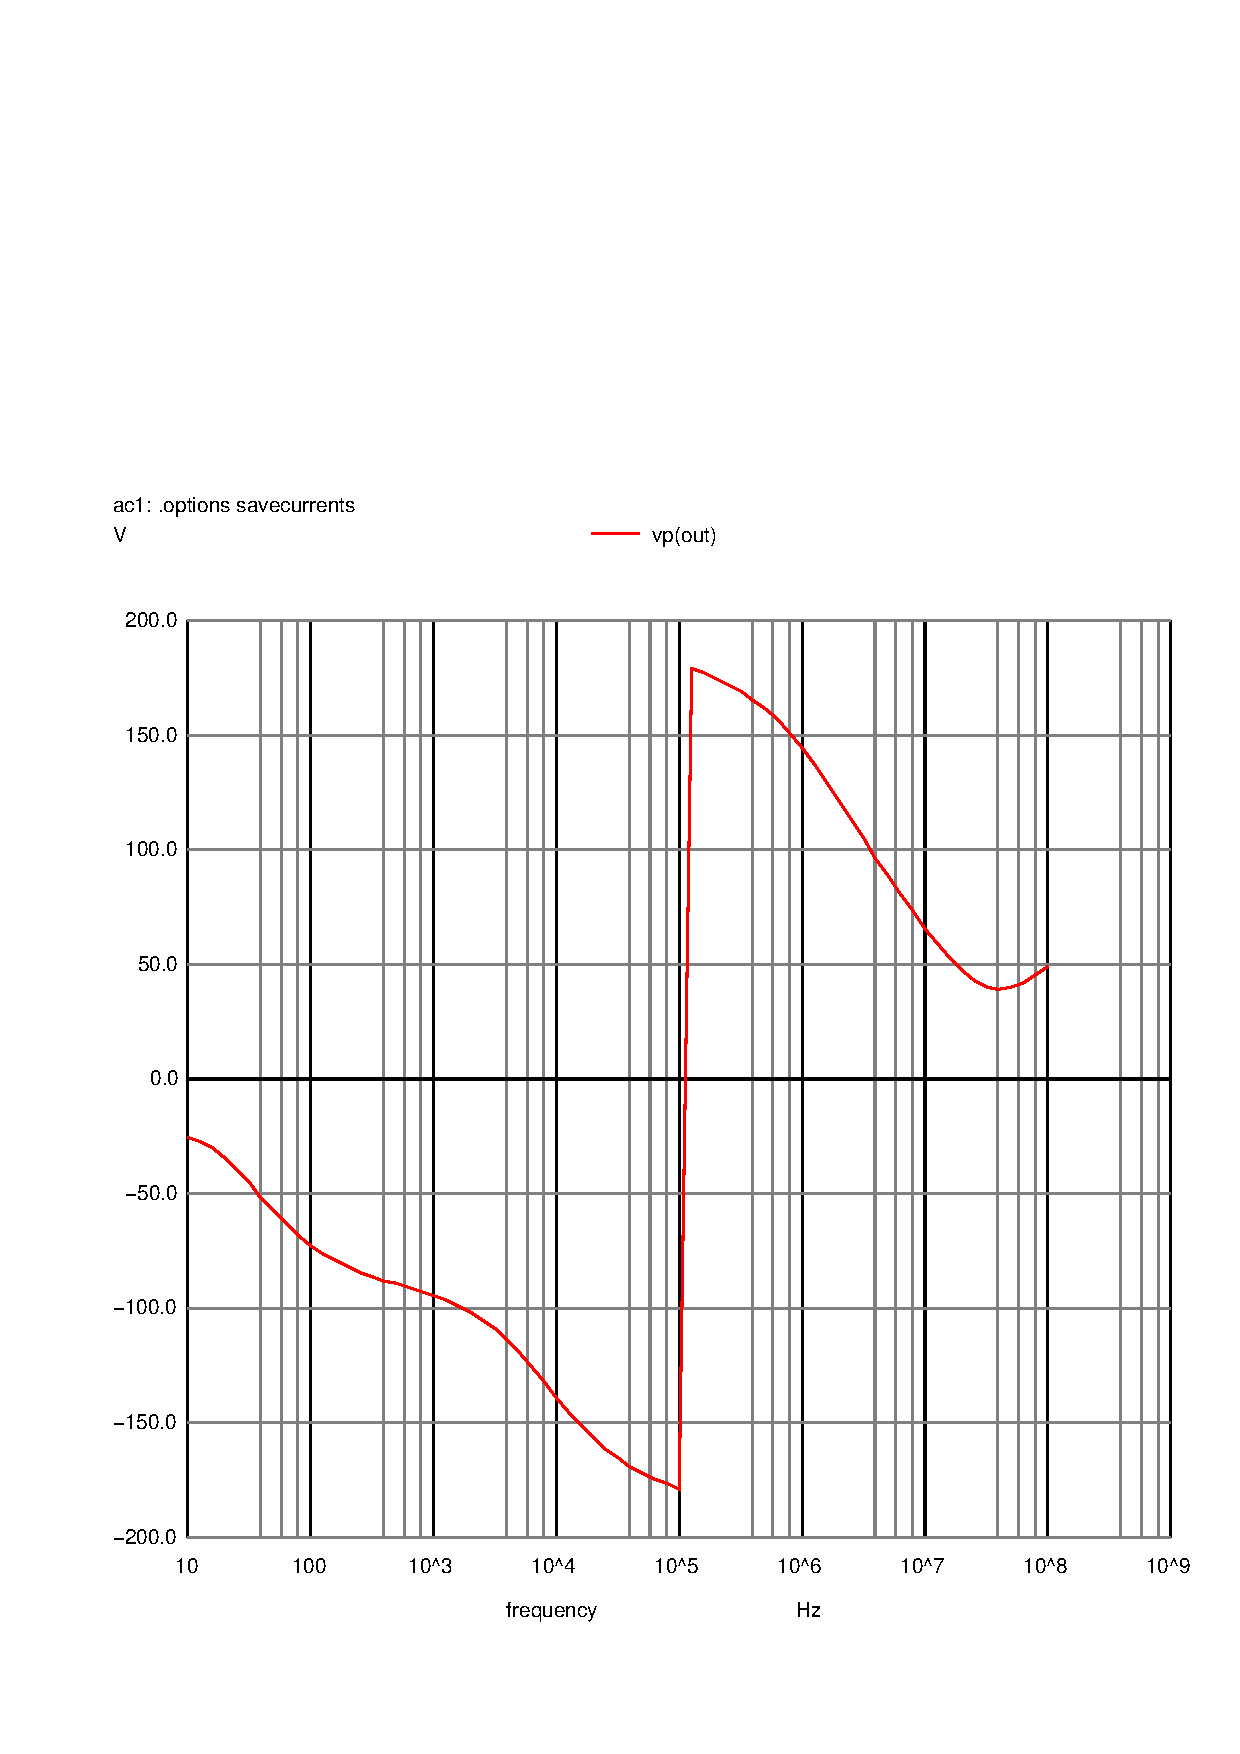
\includegraphics[width=.7\linewidth, trim={2cm 1.5cm 0.5cm 6cm}, clip]{../Simulation/vo2f_ph.pdf}
  \caption{Ngspice}
  \label{fig:PhaNG}
\end{subfigure}
\caption{Phase output}
\label{fig:Phase}
\end{figure}

\indent

After looking at both graphics it may be noticeable that the phase outputs are similar in their general shape, but differ in value. For instance, the higher cutoff frequency is located at around $10^3 Hz$ in the {\it Octave} graph and around $10^5 Hz$ in {\it Ngspice}.

 

\subsubsection*{Tables}

\begin{table}[H]
    \caption{Output parameters}
    \begin{subtable}{.5\linewidth}
      \centering
        \caption{Octave}
        \begin{tabular}{ll}
        \hline    
        {\bf Name} & {\bf Value} \\ \hline
        \input{../Analysis/OutputResults.tex}
        \end{tabular}
        \label{tab:OutParamOc}
    \end{subtable}%
    \begin{subtable}{.5\linewidth}
      \centering
        \caption{Ngspice}
        \begin{tabular}{ll}
        \hline    
        {\bf Name} & {\bf Value} \\ \hline
        \input{../Simulation/freq_tab.tex}
        \end{tabular}
        \label{tab:OutParamNG}
    \end{subtable} 
    \label{tab:OutParam}
\end{table}
\indent



\subsection{General Comments}

\indent

Looking at the data, we can confirm that the values differ by quite a margin. This is especially true for the values of the frequency.

As previously stated, the differences came from approximations such as the transistor model approximation, since its equation  was not solved. Instead models were used to calculate the voltage output.

Another source of error may come from the computation of the gain. The Magnitude plots show that the gain is quite similar, which means the frequency independent part is correct. This means the only parts which differ come from frequency dependent components. Nevertheless this could be a luck factor and the equations may be just wrong.

Finally, it is unknown why the differences appear on the OP analysis, especially on the $V_{Base}$. The computing was made with the methods described on the classes and matched the calculations made by the teacher.

